% ----------------------------------------------------------------
% Report Class (This is a LaTeX2e document)  *********************
% ----------------------------------------------------------------
\documentclass[11pt]{article}
\usepackage[english]{babel}
\usepackage{amsmath,amsthm}
\usepackage{amsfonts}
\usepackage{fancyhdr}
\usepackage{graphicx,xcolor}
\usepackage{geometry,cite}
\usepackage{pgfplots}
\usepackage{listings}
\usepackage{array}
\pgfplotsset{compat=1.18}
\fancyhead{}
\fancyfoot{}
\fancyhead[L]{\footnotesize{\textsf{Alex Cutforth | 24375019}}}
\fancyhead[R]{\footnotesize{\textsf{ENME 203, Project 2025, \today}}}
\fancyfoot[R]{\footnotesize{\textsf{page \thepage}}}
\geometry{ %showframe,               % shows frame, helpful for initial setup
           includehead,              % header
           includefoot,              % footer                "
           paper       = a4paper,    % paper format
           top         = 2.0 cm,     % margin top
           bottom      = 1.0 cm,     % margin bottom
           inner       = 2.0 cm,     % margin left (inner if "twoside")
           outer       = 2.0 cm,     % margin right (outer if "twoside")
           headheight  = 0.5 cm,     % space headline
           headsep     = 0.5 cm,     % distance header to text
           footskip    = 0.5 cm      % distance text to footer
         }
\pagestyle{fancy}
% ----------------------------------------------------------------
\begin{document}
\begin{titlepage}
\hfill
\includegraphics[width=40mm]{UCLogo.png}
\begin{center}

\vspace*{\fill}

\textbf{\huge{\textsl{Dynamics of a simplified wingsuit}}}\\
ENME203 2025 Project
\vspace*{\fill}


\textbf{\large Alex Cutforth}

\textbf{\large acu60@uclive.ac.nz}

\vspace*{\fill}

\textnormal{\large \today}

\end{center}
\end{titlepage}

% ----------------------------------------------------------------
\section*{Abstract}
This report analyses the vibration of a simple wingsuit model.
It outlines the physical shape and properties of the wingsuit, outlines the method for deriving unknown properties such as centre of mass and moment of inertia, and the process of deriving equations of motion for representing the behavior of a simple wingsuit system.
Finally, modal analysis and numerical differential equation solvers are used to test the stability of the system at different airspeeds.
It is found that placing the centre of lift infront of the centre of rotation and centre of lift can allow a wingsuit to remain stable at higher speeds than if it were designed otherwise.


% ----------------------------------------------------------------
\section*{Introduction}
This project focuses on analysing the properties of a simplified wingsuit model, this includes but is not limited to:
\begin{itemize}
  \item Kinematic analysis of significant points on the wingsuit
  \item Derivation of moments of interia, and relevant equations of motion
  \item Optimization of wingsuit properties for stability improvement
\end{itemize}
The purpose of this project is to determine which design properties are most important for ensuring a stable system in flight.
The findings may be able to serve as a set of guidlines for future wingsuit development.
According to \cite{Sepahvand2020}, skydivers have observed that wingsuits tend to start exibiting unstable behavior at around 83 m/s, so this project will find a set of conditions where the wingsuit can remain stable up to some speed greater than that.

% ----------------------------------------------------------------
\section*{Model Description}
The wingsuit side profile is based on a symmetric 1m long NACA0012 foil, as shown in Figure \ref{fig:3d_model}.
However this shape is only relevant for the derivation of Moments and Products of Inertia. The equation for this foil profile is:
\begin{equation}
  y_{foil}(x) = 5t_0(0.2969\sqrt{x}-0.126x-0.3516x^2+0.2843x^3-0.1036x^4) \label{eq:foil}
\end{equation}
where $t_0 = 0.12$ such that the length of the foil is 1m.
\\\\
The properties of the system model shown in Figure \ref{fig:sim_model} are given: \\
$k = 1500$ N/m, $k_{\theta} = 200$ Nm/rad, $d = 150$ Ns/m, $d_{\theta} = 0.03$ Nms/rad, $l_{\theta} = 0.1$ m, $l_{\alpha} = 0.05$ m, $m = 2$ kg, $C_{\theta} = 0.4$ kg/m, $C_y = 0.6$ kg/m, $L = C_{\theta}U^2\theta+C_yU\dot{y}$
\begin{figure}
  \centering
  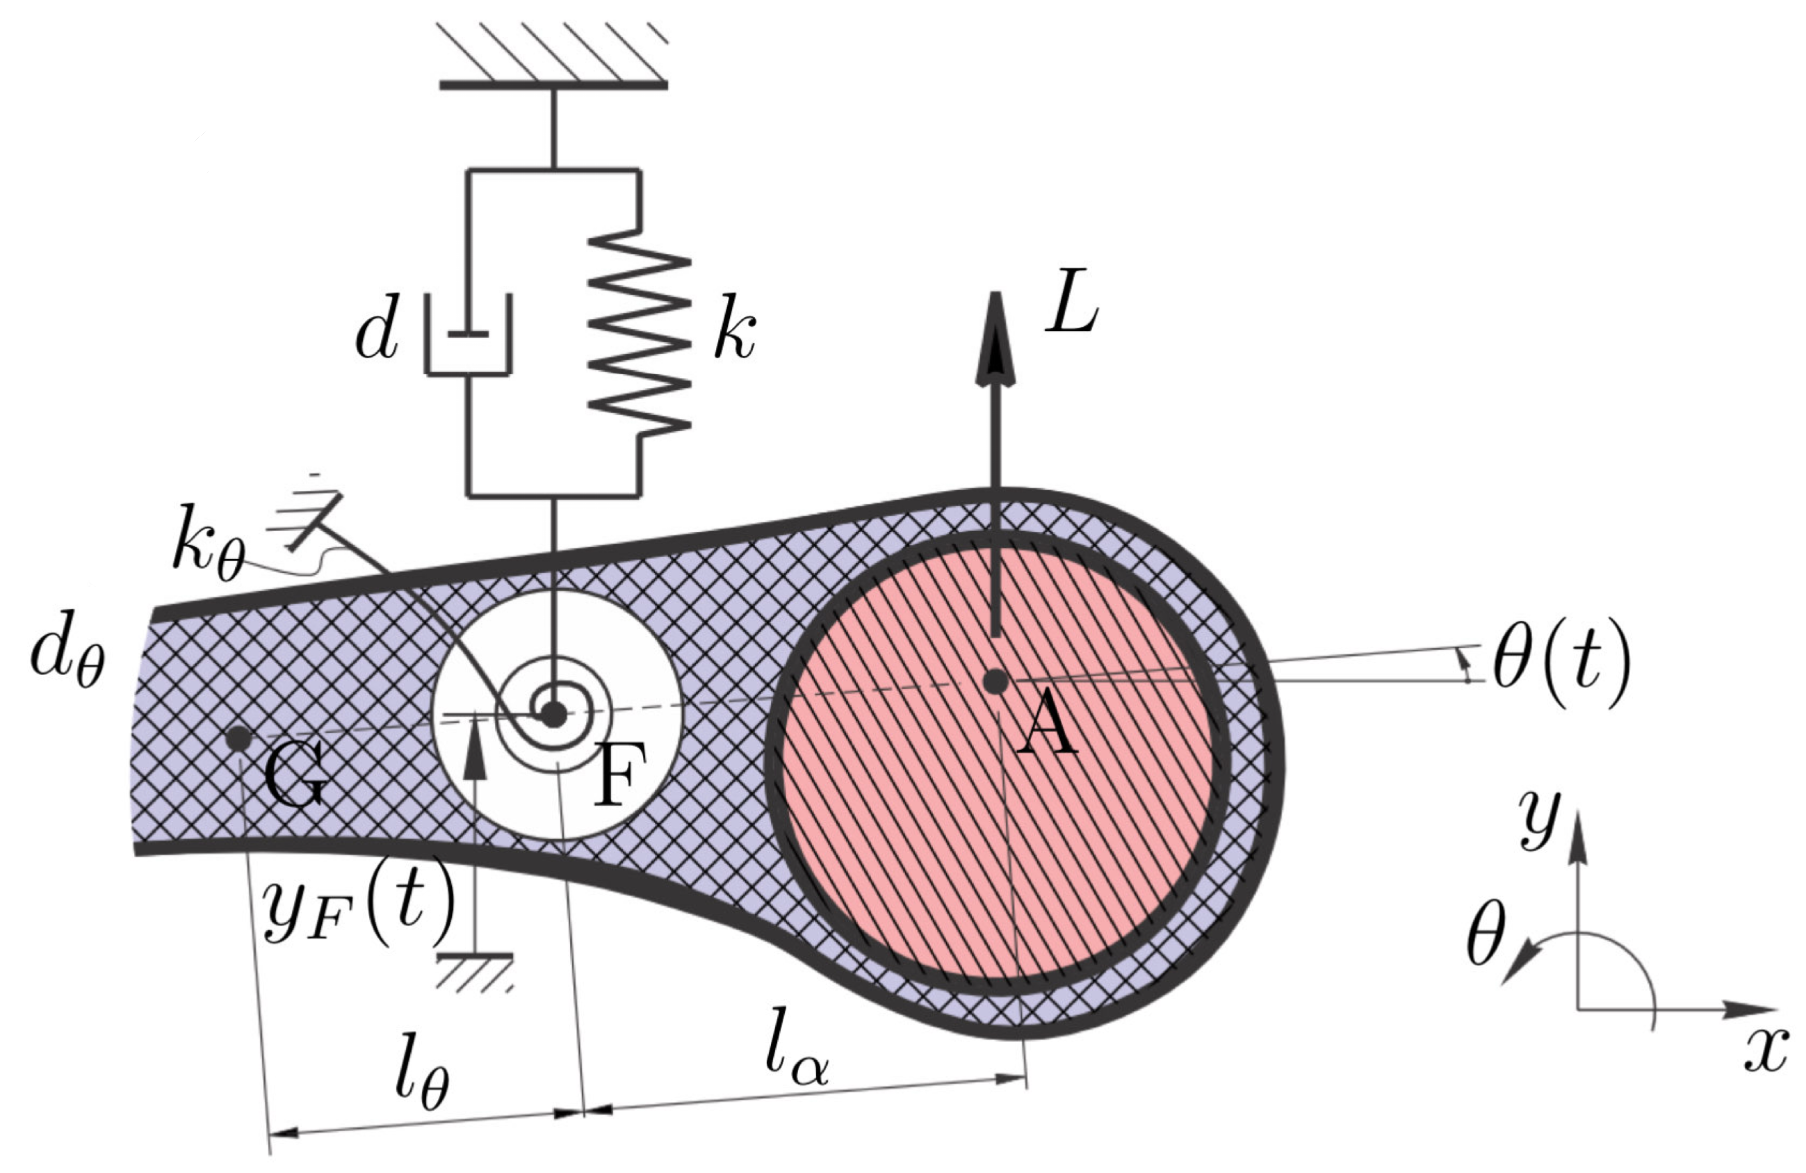
\includegraphics[width=170mm, trim=3 3 3 3, clip]{model.png}
  \caption{Simulation Model}\label{fig:sim_model}
\end{figure}

\begin{figure}
  \centering
  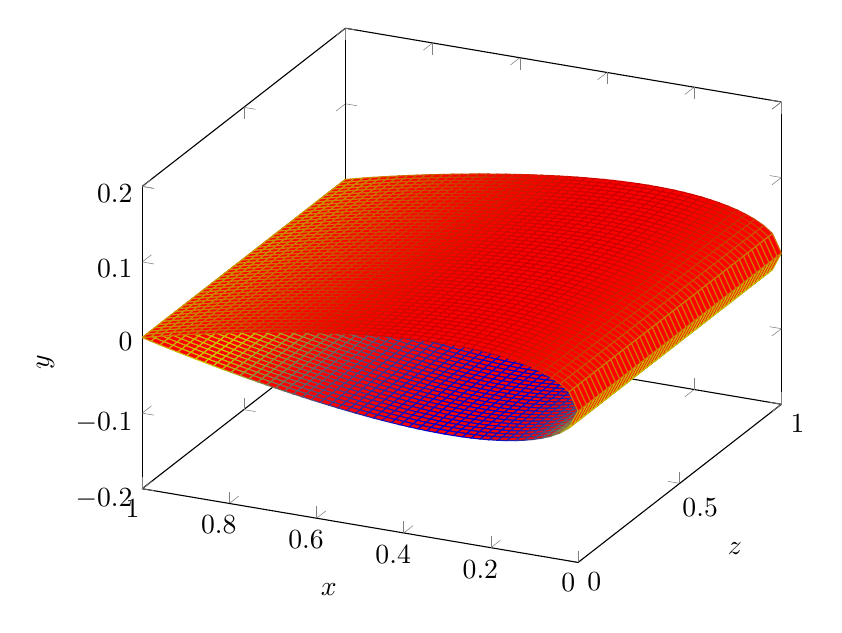
\begin{tikzpicture}
    \begin{axis}[width=0.8\linewidth, xlabel=$x$, ylabel=$z$, zlabel=$y$, zmin=-0.2, zmax=0.2, x dir = reverse]
      % These are VERY SLOW TO RENDER, so it is recommended to comment them out during writing
      \addplot3[surf, color=red, domain=0:1, samples=50]{-5*0.12*(0.2969*sqrt(x)-0.126*x-0.3516*x^2+0.2843*x^3-0.1036*x^4)};
      \addplot3[surf, color=red, domain=0:1, samples=50]{5*0.12*(0.2969*sqrt(x)-0.126*x-0.3516*x^2+0.2843*x^3-0.1036*x^4)};
    \end{axis}
  \end{tikzpicture}
  \caption{3D Foil Model}\label{fig:3d_model}
\end{figure}

% ----------------------------------------------------------------
\section*{Method}\label{sec:method}

% ----------------------------------------------------------------
\subsection*{Kinematics}\label{sec:kin}
Since the centre of rotation is not in the same place as the centre of mass for this system, it is neccessary to derive kinematic relations between angular velocities/accelerations and relative translational velocities/accelerations.
\begin{align}
  v_{G/F} &=
  \begin{pmatrix}
     \dot{\theta}l_{\theta}\sin\theta \\
    -\dot{\theta}l_{\theta}\cos\theta \\
  \end{pmatrix} \label{eq:kin1} \\
  a_{G/F} &=
  \begin{pmatrix}
     \ddot{\theta}l_{\theta}\sin\theta + \dot{\theta}^2l_{\theta}\cos\theta \\
    -\ddot{\theta}l_{\theta}\cos\theta + \dot{\theta}^2l_{\theta}\sin\theta 
  \end{pmatrix} \label{eq:kin2}
\end{align}

% ----------------------------------------------------------------
\subsection*{Dynamics}\label{sec:dyn}
\begin{align}
  m\ddot{q} &= F \nonumber \\
  m\ddot{q} &= F - d\dot{q} - kq \nonumber \\
  m\ddot{q} + d\dot{q} + kq &= F \label{eq:mdk}
\end{align}
Equation \ref{eq:mdk} is the equation of motion for a generic Mass/Dampener/Spring system, such as the one shown in Figure \ref{fig:fbd}.

\begin{figure}[h!]
  \centering
  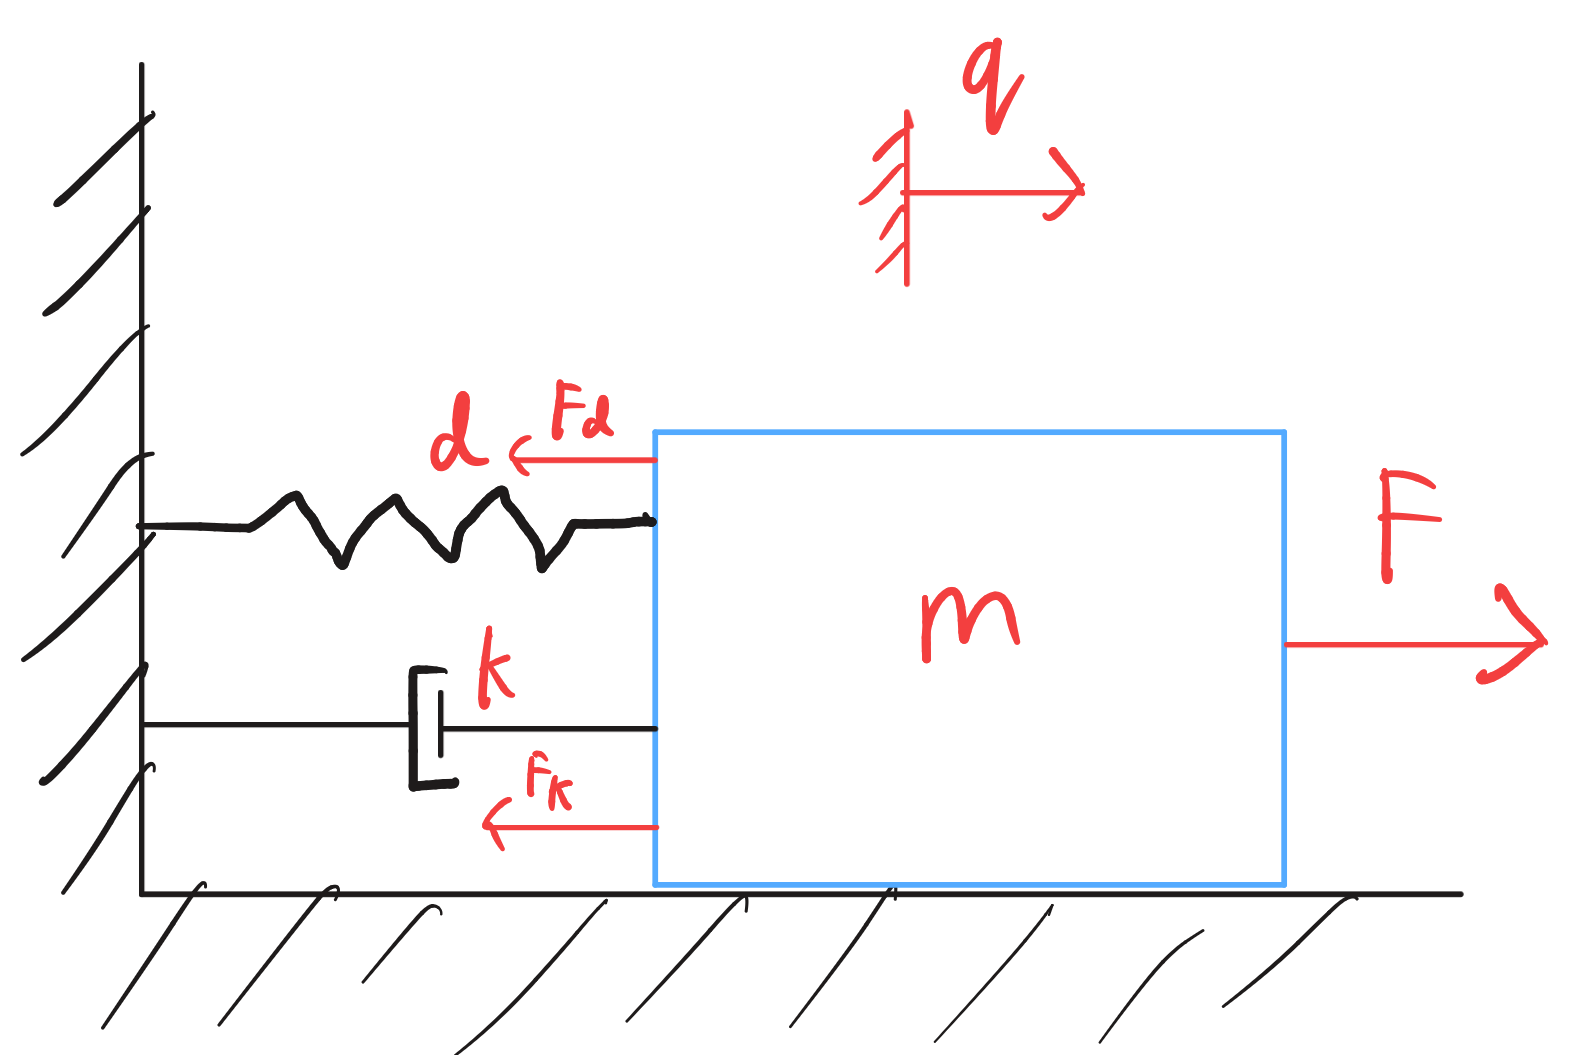
\includegraphics[width=100mm]{FBD.png}
  \caption{Generic M/D/K system Free Body Diagram}\label{fig:fbd}
\end{figure}
The wingsuit system being analysed here consists of two M/D/K systems, with the quantities $y$ and $\theta$ respectively, as shown in Figure \ref{fig:sim_model}.
\\\\
Before these equations can be applied, the moment of inertia about the flexural axis point F must be found.
Some prerequisite quantities for that are cross sectional area and centre of mass:
\begin{align*}
  A &= \int_0^{l_c}2y_{foil}(x)dx \\
    &\approx 0.0817~\mathrm{m^2} \\\\
  x_{COM} &=\frac{1}{A}\int_0^{l_c}x[2y_{foil}(x)]dx\\
    &\approx 0.4179~\mathrm{m}
\end{align*}
\textsl{Integral results are found with numerical solvers, and $y_{foil}(x)$ is defined in Equation \ref{eq:foil}}

\pagebreak
The formula for moment of inertia about the Z-axis is $\int(x^2+y^2)dm$, and applying that to the wingsuit model gives:
\begin{align*}
	I_{ZZ}^O &= \int(x^2+y^2)dm \\
    &= \int(x^2+y^2)\sigma dxdydz \\
    &= \int_0^w\sigma dz \int_0^1\int_{-y_{foil}(x)}^{y_{foil}(x)}(x^2+y^2)dydx \\
    &= \frac{m}{A}\int_0^1\int_{y_{low}(x)}^{y_{up}(x)}(x^2+y^2)dydx \\
    &\approx 0.4596~\mathrm{kgm^2}
\end{align*}
This gives the moment of intertia about the origin, which is the front tip of the wingsuit, however the quantity needed for the rotational system is moment of inertia about point F. This can be done using the parralel axis theorem $I^A=I^G+mr_g^2$.
\begin{align*}
  I^O &= I^G + mr_G^2 \\
  I^F &= I^G + mr_F^2 \\\\
  => I^F &= I^O + m(r_F^2-r_O^2) \\
    &\approx 0.1303
\end{align*}
% ----------------------------------------------------------------
\subsection*{Equation of Motion}\label{sec:eom}
Taking the generic M/D/K equation format from Equation \ref{eq:mdk} and substituting the quantities from the distinct translational and rotational systems gives us the equations of motion:
\begin{align*}
  m\ddot{y} + d\dot{y} + ky &= F \\
  I^F\ddot{\theta} + d_{\theta}\dot{\theta} + k_{\theta}\theta &= T
\end{align*}
The symbols $F$ and $T$ represent external force and torque acting upon the system, which for this model is just the lift force acting at point A.
\begin{align*}
  m\ddot{y} + d\dot{y} + ky &= L = C_{\theta}U^2\theta + C_yU\dot{y} \\
  I^F\ddot{\theta} + d_{\theta}\dot{\theta} + k_{\theta}\theta &= l_{\alpha}L = l_{\alpha}(C_{\theta}U^2\theta + C_yU\dot{y})
\end{align*}
Then, since the centre of rotation is not in the same location as the centre of mass, the equations must be linearized, giving the final equations of motion:
\begin{align}
  m\ddot{y} - ml_{\theta}\ddot{\theta} + d\dot{y} + ky &= L = C_{\theta}U^2\theta + C_yU\dot{y}\label{eq:eom1} \\
  I^F\ddot{\theta} - ml_{\theta}\ddot{y} + d_{\theta}\dot{\theta} + k_{\theta}L &= l_{\alpha}\theta = l_{\alpha}(C_{\theta}U^2\theta + C_yU\dot{y})\label{eq:eom2}
\end{align}
This is a 2 degrees of freedom system, hence why there are two seperate equations of motion. This is because the translational and rotational properties of the system are not completely dependent upon each other. However, they are \textsl{partially} dependent, which is why there is sharing of quantities between equations. These are known as coupled equations.

% ----------------------------------------------------------------
\section*{Analysis \& Discussions}\label{sec:anal_disc}
\subsection*{Decoupled Analysis}\label{sec:decoupled_analysis}
As stated in the Dynamics section, the equations of motion for this system are coupled, this means the equations can not be analysed induvidually, but rather as a system of differential equations.
However, it is possible to set specific conditions where the equations decouple from each other, this occurs when the centre of mass and flexural axis are aligned ($l_{\theta} = 0$), and the lift coefficient associated with the equation in question's quantity is set to zero ($C_y$ or $C_{\theta} = 0 $). \\\\
Case 1, substituting $l_{\theta} = 0$ and $C_y = 0$ into Equation \ref{eq:eom2} gives:
\begin{equation}
  \ddot{\theta}+\frac{d_{\theta}}{I^F}\dot{\theta}+\frac{k_{\theta}-l_{\alpha}C_{\theta}U^2}{I^F}\theta = 0 \label{eq:decoupled1}
\end{equation}
This equation can then be considered with the format $\ddot{q} + 2\zeta\omega\dot{q}+\omega^2q = 0$, giving:
\begin{align*}
  \omega &= \sqrt{\frac{k_{\theta}-l_{\alpha}C_{\theta}U^2}{I^F}} \quad \mathrm{(Angular~Frequency)} \\
  \zeta &= \frac{d_{\theta}}{2\sqrt{I^F(k_{\theta}-l_{\alpha}C_{\theta}U^2)}} \quad \mathrm{(Damping~Ratio)}
\end{align*}
This information allows us to find a critical airspeed where the wingsuit's torsional mode becomes statically unstable.
This critical airspeed occurs when the real component of the roots (given by $\lambda = -\zeta\omega\pm i\omega\sqrt{1-\zeta^2}$) of the equation of motion equal zero.
Given a positive value for $d_{\theta}$, the equation for $\zeta$ cannot be zero, so to find the solution, $\omega$ must be set to zero. This gives:
\begin{align*}
  k_{\theta} &= l_{\alpha}C_{\theta}U^2 \\
  U &= \sqrt{\frac{k_{\theta}}{l_{\alpha}C_{\theta}}}\\
    &= 100~\mathrm{m/s}
\end{align*}
Which is further demonstrated in Figure \ref{fig:decoupled_case1}
\begin{figure}[h!]
  \centering
  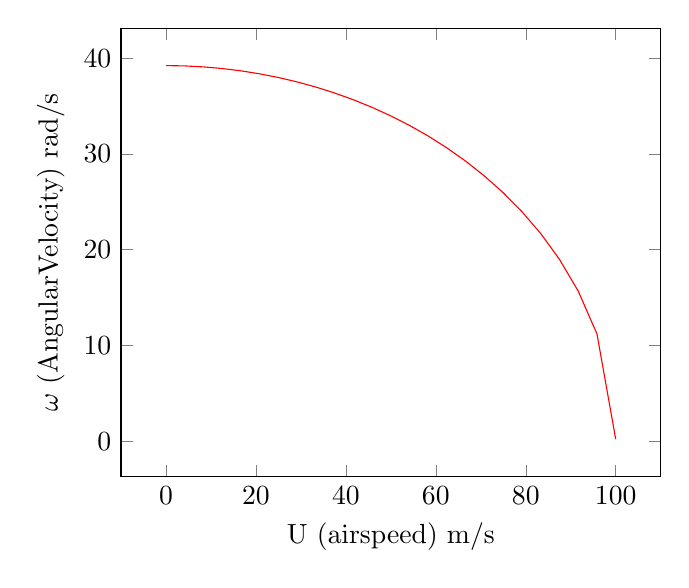
\begin{tikzpicture}
    \begin{axis}[xlabel=U (airspeed) m/s, ylabel=$\omega~\mathrm{(Angular Velocity)~rad/s}$]
      \addplot[color=red, domain=0:100]{sqrt((200 - 0.05 * 0.4 * x^2) / 0.13)};
    \end{axis}
  \end{tikzpicture}
  \caption{Graph showing x-intercept of angular velocity}\label{fig:decoupled_case1}
\end{figure}
\\\\
Case 2, substituting $l_{\theta} = 0$ and $C_y = 0$ into Equation \ref{eq:eom1} gives:
\begin{equation}
  \ddot{y}+\frac{d-C_yU}{m}\dot{y}+\frac{k}{m}y = 0
\end{equation}
And again, using the format $\ddot{q} + 2\zeta\omega\dot{q}+\omega^2q = 0$ gives the equations:
\begin{align*}
  \omega &= \sqrt{\frac{k}{m}} \\
  \zeta &= \frac{d-C_yU}{2\sqrt{km}}
\end{align*}
To find the condition where the real component of the roots is zero, $\zeta$ must be zero, since $\omega$ cannot be zero in this case (unless the spring is removed, such that $k = 0$, but that is a trivial case to be ignored).
\begin{align*}
  U  &= \frac{d}{C_y} \\
  &= 250 ~\mathrm{m/s}
\end{align*}
The y-intercept to show this is given in Figure \ref{fig:decoupled_case2}, and evidence of stable and unstable oscillation is shown in Figure \ref{fig:decoupled_solution}
\begin{figure}[h!]
  \centering
  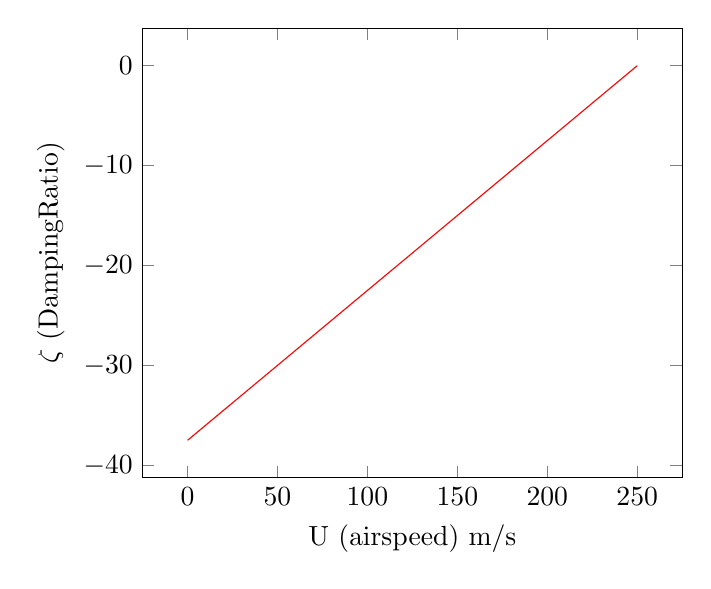
\begin{tikzpicture}
    \begin{axis}[xlabel=U (airspeed) m/s, ylabel=$\zeta~\mathrm{(Damping Ratio)}$]
      \addplot[color=red, domain=0:250]{(0.6 *x - 150)/4};
    \end{axis}
  \end{tikzpicture}
  \caption{Graph showing x-intercept of damping ratio}\label{fig:decoupled_case2}
\end{figure}
\begin{figure}[h!]
  \centering
  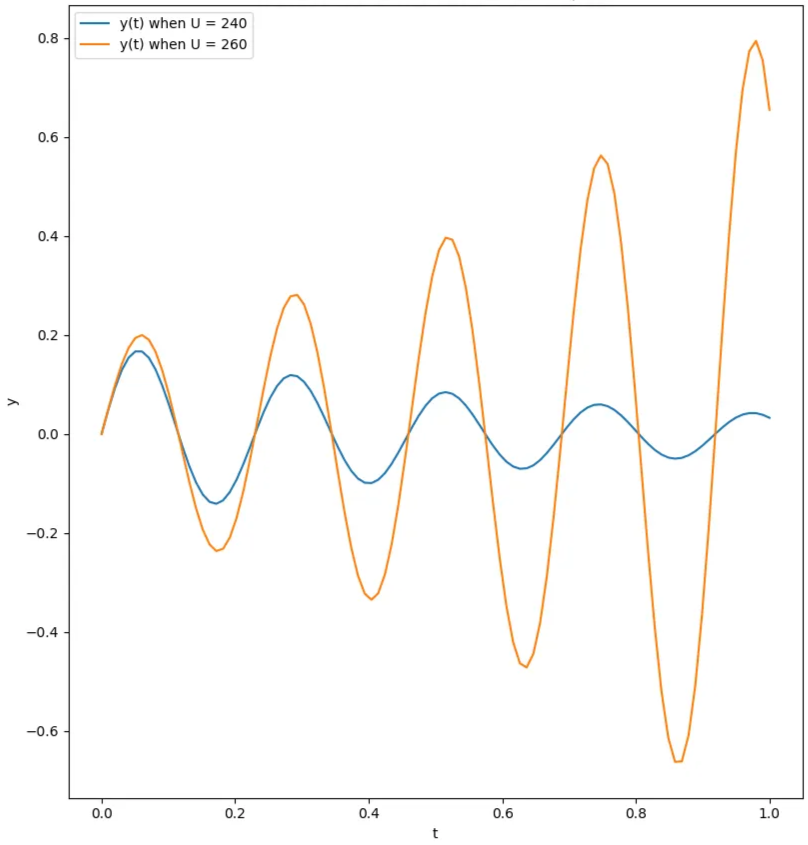
\includegraphics[width=100mm]{decoupled_solution.png}
  \caption{Solutions to oscillation of y over 1 second on either side of critical airspeed}\label{fig:decoupled_solution}
\end{figure}


\subsection*{Modal Analysis}\label{sec:modal_analysis}
Modal analysis allows us to see the stability of the system as a whole when both degrees of freedom are partially interacting.
To analyse both equations of motion simultaneously they can be represented in a matrix system of the form:
$$
  \mathbf{M}\ddot{X}+\mathbf{D}\dot{X}+\mathbf{K}X = 0
$$
Then substituting in equations \ref{eq:eom1} and \ref{eq:eom2}
$$
  \overbrace{
    \begin{bmatrix}
      I^F&-ml_{\theta} \\
      -ml_{\theta}&m
    \end{bmatrix}
  }^{\mathbf{M}}
  \overbrace{
    \begin{bmatrix}
      \ddot{\theta} \\
      \ddot{y}
    \end{bmatrix}
  }^{\ddot{X}}
  +
  \overbrace{
    \begin{bmatrix}
      d_{\theta}&-l_{\alpha}C_yU\\
      0&d-C_yU
    \end{bmatrix}
  }^{\mathbf{D}}
  \overbrace{
    \begin{bmatrix}
      \dot{\theta} \\
      \dot{y}
    \end{bmatrix}
  }^{\dot{X}}
  +
  \overbrace{
    \begin{bmatrix}
      k_{\theta}-l_{\alpha}C_{\theta}U^2&0\\
    -C_{\theta}U^2&k
    \end{bmatrix}
  }^{\mathbf{K}}
  \overbrace{
    \begin{bmatrix}
      \theta \\
      y
    \end{bmatrix}
  }^X
  = 0
$$
This system can then be converted into state space.
\begin{align*}
  \begin{bmatrix}
    I&0\\
    0&M
  \end{bmatrix}
  \begin{bmatrix}
    \dot{X}\\
    \ddot{X}
  \end{bmatrix}
  +
  \begin{bmatrix}
    0&-I\\
    K&D
  \end{bmatrix}
  \begin{bmatrix}
    X\\
    \dot{X}
  \end{bmatrix}
  &=0
  \\
  \frac{d}{dt}
  \begin{bmatrix}
    X\\
    \dot{X}
  \end{bmatrix}
  &=
  \begin{bmatrix}
    0&I\\
    -K&-D
  \end{bmatrix}
  \begin{bmatrix}
    I&0\\
    0&M
  \end{bmatrix}^{-1}
  \begin{bmatrix}
    X\\
    \dot{X}
  \end{bmatrix}
\end{align*}
This system is suitable for use with an initial value problem numerical solver, and the stability can be determined by finding the eigenvalues of the coefficient matrix (see Figure \ref{fig:modal_roots} and Appendix A).
$$
  A = 
  \begin{bmatrix}
    0&I \\
    -K&-D
  \end{bmatrix}
  \begin{bmatrix}
    I&0 \\
    0&M
  \end{bmatrix}^{-1}
$$
\begin{figure}[h!]
  \centering
  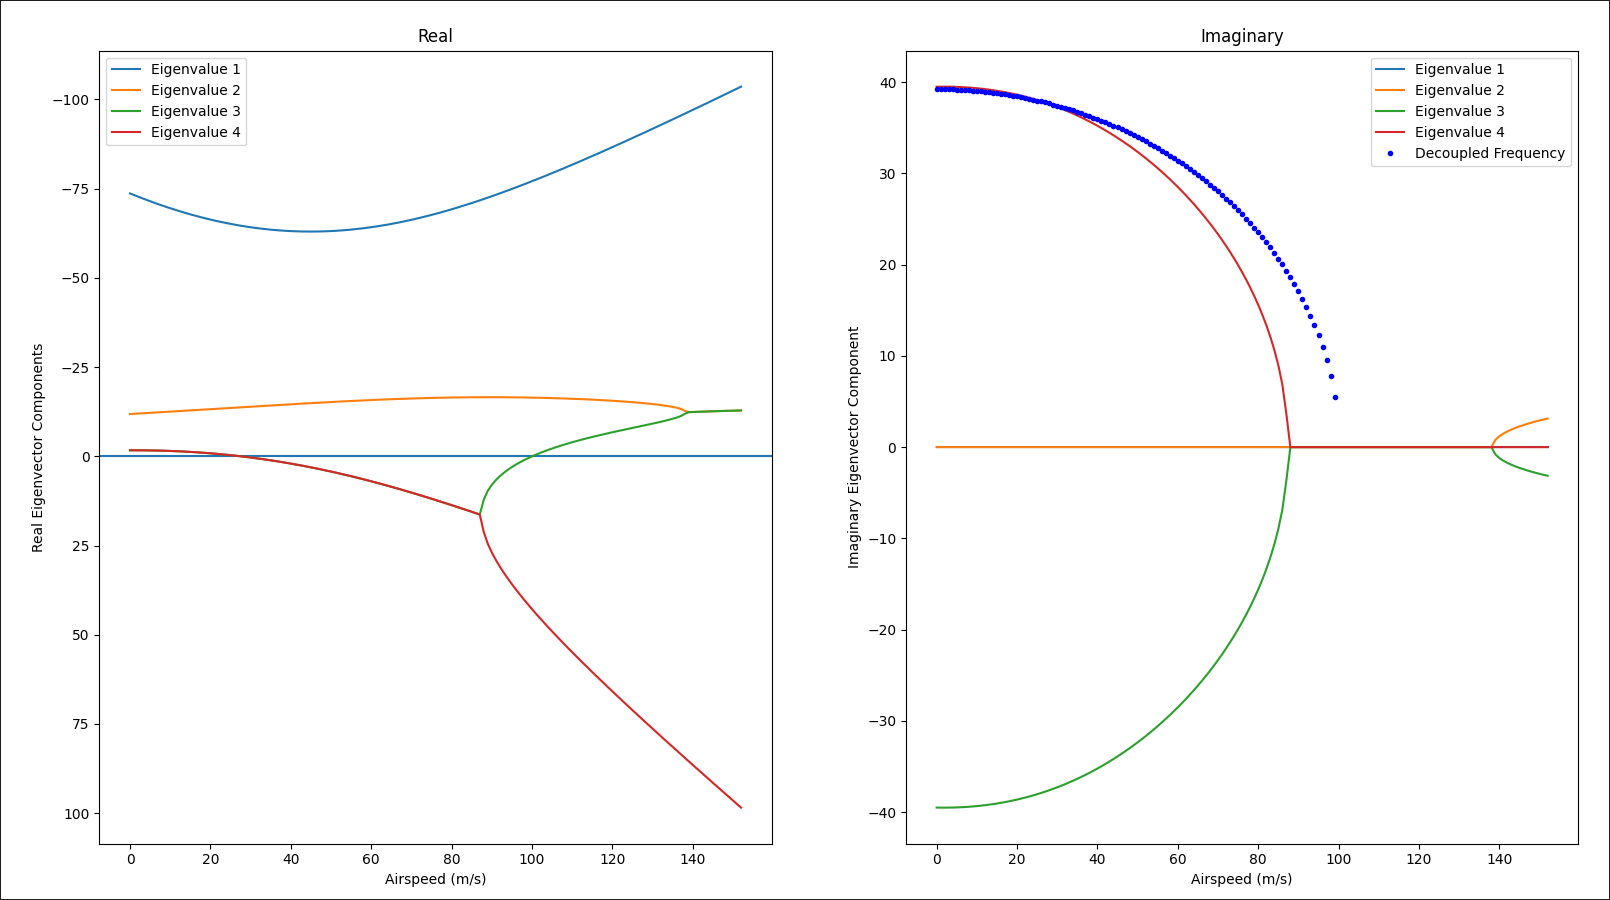
\includegraphics[width=170mm, trim=3 3 3 3, clip]{modal_roots.png}
  \caption{Unoptimized Modal Roots}\label{fig:modal_roots}
\end{figure}
A system is unstable if the real parts of any of its eigenvalues is postive, and Figure \ref{fig:modal_roots} shows that the system has positive real components for approximately $U > 30$ m/s, meaning this wingsuit model looses stability above that velocity. This is a relatively low speed for general wingsuit flight, so this must be improved.
\\\\
Through some trial and error, it was found that putting the centre of lift behind the centre of gravity, by making $l_{\theta}$ negative, and decreasing the size of $l_{\alpha}$, the system remains stable into much higher airspeeds. This is shown in Figure \ref{fig:optimized_system} (the vertical line in the graph of real components is a reference velocity of 92m/s or 330km/h).
\\\\
While this analysis can shed light on the general behavior of properties of a wingsuit, this method of analysis is unlikely to yield accurate predictions of the behavior of a real wingsuit in flight, as it is ignoring many aerodynamic phenomena which can impact the inflight behavior, such as air turbulence, vortices, and other external forces not parralel with the vertical axis. Further research could include comprehensive aerodynamic simulations or even Finite Element Analysis on the foil to determine what effects the system vibrations may have on the integrity of the wing structure.
\begin{figure}[h!]
  \centering
  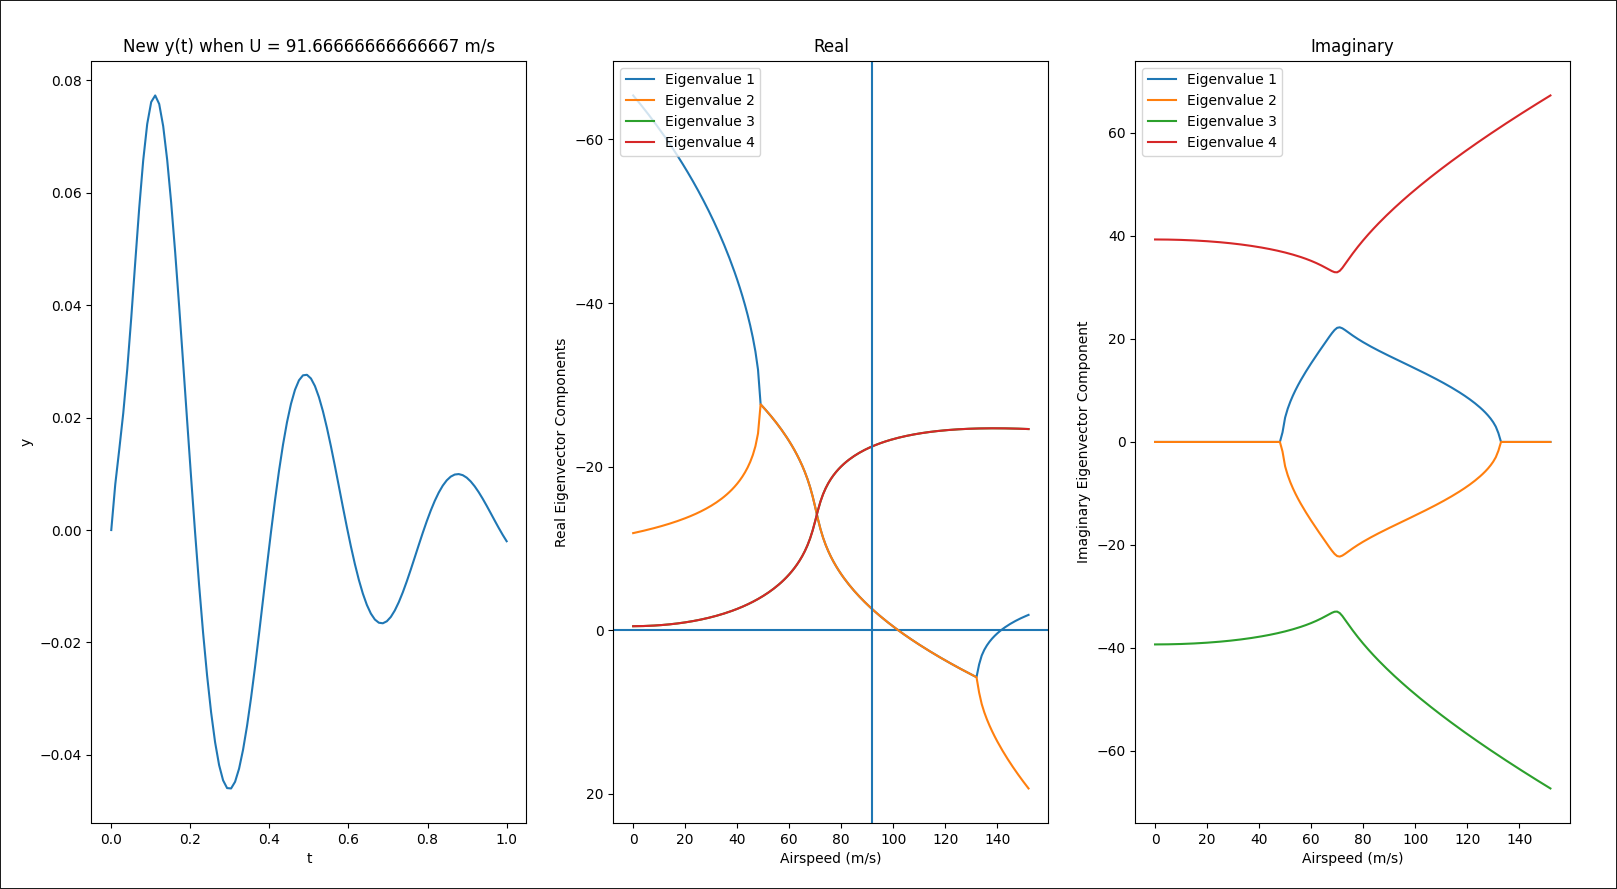
\includegraphics[width=170mm, trim=3 3 3 3, clip]{optimized_system.png}
  \caption{Optimized System}\label{fig:optimized_system}
\end{figure}

% ----------------------------------------------------------------
\section*{Conclusions}\label{sec:conclusion}
This report outlined the process for determening the properties of a standard NACA foil, and deriving the equations of motion for translational and rotational movement in a wingsuit.\
Using these equations, a method for analyzing the stability of the system was found using linear algebra and numerical analysis.
Based on this analysis the initial properties of the wingsuit model were optimized to increase the maximum stable airspeed for the wingsuit. This was done by shifting the centre of mass to be infront of the centre of lift and flexural axis.
Further research should be done to validate this analysis through the use of aerodynamic simulations to help understand the influence of airflow around the wingsuit on the stability of the system.

% ----------------------------------------------------------------
\bibliography{project}{}
\bibliographystyle{unsrt}

\pagebreak
\section*{Appendix A}\label{sec:code}
\lstinputlisting[language=Python, caption=Wingsuit Modeling Script]{wingsuit.py}
\pagebreak
\thispagestyle{empty}
\section*{Declaration of Use for Generative AI in Assessments \quad 
\includegraphics[width=30mm]{UCLogo.png}}
\begin{center}

\begin{tabular}{|c|c|}
  \hline
  Full Name & Alexander James Cutforth \\
  \hline
  Student ID Number & 24375019 \\
  \hline
  Student Email & acu60@uclive.ac.nz \\
  \hline
  Course Code & ENME203 \\
  \hline
  Assessment Name & Project Part 3 Communication Skills \\
  \hline
\end{tabular}
\subsection*{Acknowledgement of Assessment Submission}
I, Alex Cutforth, hereby confirm that on \today:
\begin{enumerate}
  \item The document I have submitted was written by me.
  \item When using AI, I have ensured that the work produced is still my own and I understand that submitting output from a generative AI tool as my own is NOT acceptable.
  \item To assist with maintaining academic integrity, I have appropriately acknowledged any use of generative AI in my work (list below as applicable).
  \item I acknowledge that any undeclared use of generative AI will constitute academic dishonesty and will be dealt with according to relevant University policy.
  \item I understand that I will be held accountable and liable for any academic misconduct that arises in breach of any relevant University policy, as well as the consequences of such infringements.
\end{enumerate}
\subsection*{Acknowledgement of Generative AI Tools Used}
\begin{tabular}{|m{3cm}|m{3cm}|m{10cm}|}
  \hline
  AI Tool Used & Purpose of Use & Briefly Explain the Extent of Use \\
  \hline
  Claude Sonnet 4.5 & Write a Python function & I used it to write a function which was used for sorting eigenvalues after finding them numerically. This behavior is not required for the project nor is it taught in the course, but the plotted graphs of eigenvalue components were much harder to read previously as the colourcoding does not work properly without sorting them. The function in question has an acknowledgement of this commented above it.\\
  \hline
\end{tabular}

\end{center}

\end{document}
% ----------------------------------------------------------------
